\documentclass{article}
\usepackage{amsfonts, amsmath, amssymb, amsthm} % Math notations imported
\usepackage{enumitem}
\usepackage{graphicx}
\usepackage[margin=1in]{geometry}
\usepackage{setspace}
\graphicspath{{./images/}} % Path to images

% \begin{figure}[htb!]
%      \centering
%      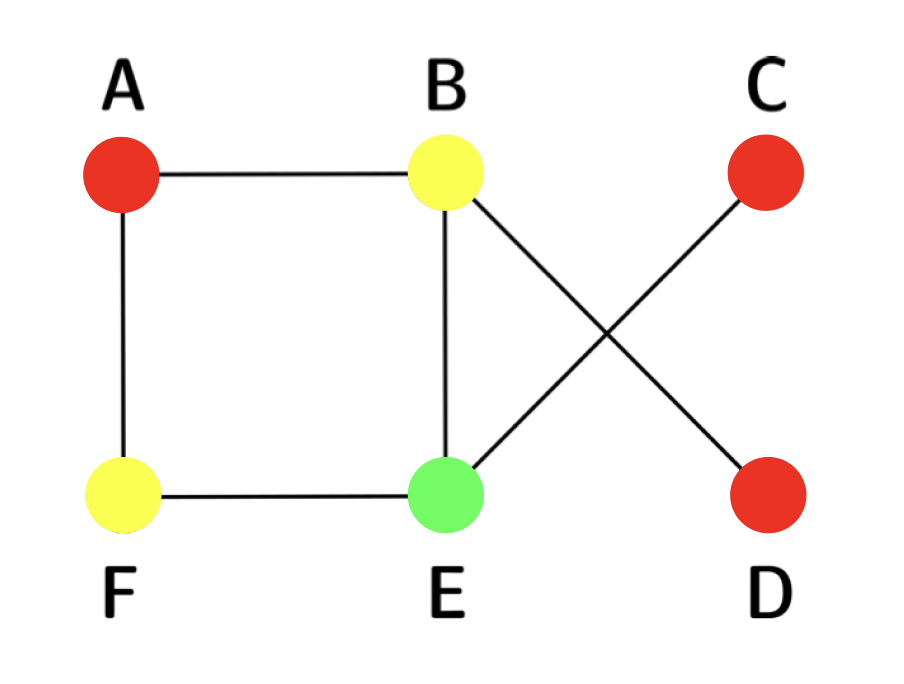
\includegraphics[scale=0.5]{coloring.png}
%      \caption{Coloring of the graph.}
% \end{figure}

\newtheorem{thm}{Theorem}
\newtheorem{proposition}[thm]{Proposition}
\newtheorem{cor}[thm]{Corollary}

% title information
\title{Math 110 HW1}
\author{Neo Lee}
\date{09/02/2023}

\setstretch{1.15}
% main content
\begin{document} 

% placing title information; comment out if using fancyhdr
\maketitle 

\section*{Problem 1}
Determine which complex numbers $x$ satisfy the equation $x^3 + x^2 + x + 1 =0$.

\section*{Problem 2}
Does there exist a complex number $\lambda$ such that $\lambda (2-3i, 5+4i, -6+7i) = 
(2+i, 3-i, 4)$?

\section*{Problem 3}
Suppose that $\{0, 1, x\}$ is a field with exactly three elements. What do the addition and 
multiplication tables have to be in that case? Based on the addition and multiplication tables you 
get, check this is indeed a field. What is the 'natural' way to think of this field (and of x)?


\section*{Problem 4}
Suppose $a$ is a fixed real number, and consider the set of all real-valued twice differential 
functions $f$ on the interval $[0, \infty)$ such that $f''(2) + af'(1) - af(0) = 2a$ (equipped with 
the usual addition of functions and multiplication by real scalars). For which values of a is this 
a vector space over $\mathbb{R}$?

\section*{Problem 5}
Suppose $S$ is a non-empty set and $V$ is a vector space. Let $V^S$ denote the set of functions from 
$S$ to $V$. Define a natural addtion and scalar multiplication on $V^S$, and show that $V^S$ is a 
vector space with these definitions.

\end{document}
